%\label{subsec:story-mining}

In a software development scenario, project participants add, remove, modify and perform several different operations in an artifact and store these changes in a shared repository (such as GitHub or Subversion). Different participants may change an artifact, and therefore it is a collaborative work towards a final product. Moreover, they can add comments when committing changes to an artifact bringing insights of the working process performed in this artifact.

We argue that these comments 
%form the textual elements is a kind of story being told, with additional elements such as location (the specific folder and files being manipulated at the broader view of a Project folder tree map) and the timestamp of their specific operation. The comments text and the additional elements
follow a similar structure of the story applied at the Story Mining method  \cite{Goncalves2011} , i.e., the comments provided by the different participants build the story about the work being done in the particular artifact. Moreover, additional elements such as time of the commit and the project participant responsible for the changes provide extra information that can be used to represent the artifact evolution. Therefore, in this research we use story mining to build a process which represents the artifact evolution. The input of the story mining is a set artifact stories, where the story of the \emph{i}-th artifact is obtained from the set $AE$ of aggregated events as $ story({f_i}) = \lbrace {m ~|~ a_e \in AE,~ f(a_e) = f_i,~ ak(a_e)=m} \rbrace$.


%several distinct visualizations from these stories to represent the software process elements, thus depicting critical viewpoints for the participants.
For instance, consider information about $4$ aggregate events related to a specific artifact as depicted in \Cref{table:ExampleOfComments}:

\begin{table}[!h]
	\caption{Comments made by project participants in four different times when committing changes performed in a artifact.}
	\label{table:ExampleOfComments}
\begin{center}
\begin{tabular}{|c|c|l|}
Time & Project Participant & Comment\\\hline
$ats_1$ & $au_1$ & Add requirements file. \\
$ats_2$ & $au_2$ &Update requirements.\\
$ats_3$ & $au_2$ &Modify requirements.\\
$ats_4$ & $au_2$ &Specify solved time for problem.\\
\end{tabular}
\end{center}
  
\end{table}

Using the story mining approach we are able to find the process activities. Then, considering the time of each commit, a workflow is created. Moreover, we associated the participant responsible for the work as the one that committed the changes. The final process discovered for the illustrative example is depicted in Figure \ref{fig:ExampleOfWorkingProcess}.

\begin{figure}[!h]
	\centering
  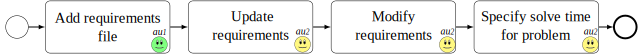
\includegraphics[width=.9\linewidth]{ProcessExample}
  \caption{Working process generated from the set of comments depicted in Table
  \label{fig:ExampleOfWorkingProcess} \ref{table:ExampleOfComments}. The color images represent the user responsible for the commit.}
\end{figure}


